\section{Implementation of a Parametetric SABR Model and Implicit Neural Network Architectures}
\label{sec:implementation}

\subsection{Defining the SABR Model Equations}
\label{subsec:sabr}
The SABR model is a stochastic differential model, defined by the following equations in which the dynamics of the
asset price and the corresponding volatility levels are used to calculate an approximation to the implied volatility where no contract is traded.
\begin{itemize}
    \item \textbf{Alpha (\(\alpha\))}: This is the initial volatility level.
    \item \textbf{Beta (\(\beta\))}: The elasticity parameter between the volatility of the asset and its price.
    \item \textbf{Rho (\(\rho\))}: Statistical correlation between the asset price and its volatility, also called \textit{spot-volatility correlation}.
    \item \textbf{Volvol (\(\nu\))}: The volatility of the volatility process itself.
\end{itemize}

The implied volatility function of the SABR model is then given by:

\begin{equation}
    \label{eq:sabr}
    \sigma_{\textit{BS}}(f, K) =
    \alpha \frac{(fK)^{\frac{1 - \beta}{2}}}{1 + \left(\frac{(1 - \beta)^2 \rho^2}{24} + \frac{(1 - \beta)^2(2 - 3\rho^2)}{1920} \right) (fK)^{1 - \beta}}
\end{equation}

In the context of this paper, multiple SABR models are used daily, one for each unique strike price per day.
Three continuous functions are used to map from continuous maturities to three model parameters: $\alpha$, $\rho$, and $\nu$.
This is done to allow for a smooth transition between the different strike levels,
as using a single SABR model by itself is known to not be able to replicate observed implied volatility surfaces~\cite{Hagan2015, Kim2021}.
Given the functions for the parameters $\alpha_t = f_{\alpha}(t, \textbf{P})$, $\rho_t = f_{\rho}(t, \textbf{Q})$, and $\nu_t = f_{\nu}(t, \textbf{R})$ (values for $\beta$ are fixed and remain unchanged),
and the encoding variables \textbf{P, Q}, and \textbf{R} respectively, such that $\textbf{P} \in \mathbb{R}^{5}$, $\textbf{Q} \in \mathbb{R}^{4}$, and $\textbf{R} \in \mathbb{R}^{4}$,
the daily parameters for the SABR model are obtained by the following equations for any continuous value of $t$:

\begin{equation}
    \label{f_alpha}
    f_{\alpha}(t, \textbf{P}) = P_0 + \frac{p_3}{P_4} \left( \frac{1 - e^{-P_4 t}}{P_4 t} \right) + \frac{P_1}{P_2} e^{-P_2 t}
\end{equation}
\begin{equation}
    \label{f_rho}
    f_{\rho}(t, \textbf{Q}) = Q_0 + Q_1 t + Q_2 e^{-Q_3 t}
\end{equation}
\begin{equation}
    \label{f_nu}
    f_{\nu}(t, \textbf{R}) = R_0 + R_1 t^{R_2} e^{R_3 t}
\end{equation}

Therefore, the task becomes obtaining the encoding variables \textbf{P}, \textbf{Q}, and \textbf{R} for daily SABR models.
Initially, we use the Broyden-Fletcher-Goldfarb-Shanno (\textit{BFGS} ) algorithm to fit the encoding variables
that best minimize the mean absolute error (MAE) between the observed implied volatilities and corresponding SABR generated implied volatilities.
The resulting SS scores are then calculated as the MAE between the fitted $f_{\alpha}(t, \textbf{P})$, $f_{\rho}(t, \textbf{Q})$, $f_{\nu}(t, \textbf{R})$
and the fitted values for $f_{\alpha}(t, \widetilde{\textbf{P}})$, $f_{\rho}(t, \widetilde{\textbf{Q}})$, and $f_{\nu}(t, \widetilde{\textbf{R}})$,
where $\widetilde{\textbf{P}}$, $\widetilde{\textbf{Q}}$, and $\widetilde{\textbf{R}}$ are the encoding variables
obtained using a subset of the daily candidate according to a Monte Carlo selection
detailed in \hyperref[subsubsec:monte_carlo]{Section~\ref*{subsubsec:monte_carlo}},
similarly to the selection a human trader would make when selecting the most relevant data points to fit the SABR parameters
to reduce arbitrage opportunities~\cite{Kim2021}.
A visual representation of a surface with an arbitrage opportunity is shown in \hyperref[fig:figure3]{Figure~\ref*{fig:figure3}}.
Finally, the neural network is trained to predict the SS scores for each candidate point $\mathcal{S}_{i}^{t} \in \mathcal{S}^{t}$ from the daily observed input.
The task can then be classified as a supervised regression task and a
Root Mean Squared Error (RMSE) between the transformer predicted SS scores and those calculated using the Monte Carlo estimation
is used as loss score\footnote{The RMSE between the SS scores is not to be confused with the MAE between the calculated SABR parameters.
The first is used as the loss function when training the neural network model,
    while the second is used as the BFGS objective function when optimizing for the encoding variables that best replicate the observed daily surface.}.

\begin{figure}[h]
    \begin{center}
        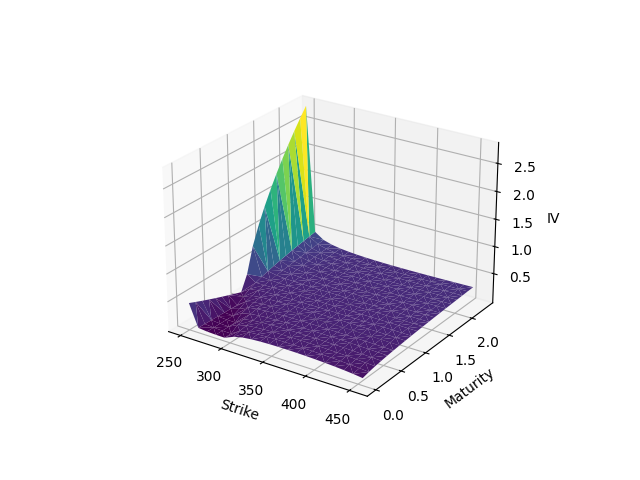
\includegraphics[width=0.4\textwidth]{images/unfitted}
        \caption{Surface generated using SABR models fit on entire candidate set, resulting in an outlier peak.}
        \label{fig:figure1}
    \end{center}
\end{figure}

\subsection{Proposed Architecture}
\label{subsec:architecture}

As mentioned, transformers are capable of capturing complex dependencies in sequential non-fixed length data.
Within our proposed architecture, we use a transformer encoder to approximate the \textit{SS} scores
for each candidate point $\mathcal{S}_{i}^{t} \in \mathcal{S}^{t}$ from the daily observed input.

\subsubsection{Details on the Chosen Transformer Encoder}

Unlike recurrent neural networks (RNNs) and convolutional neural networks (CNNs), transformers do not rely on a fixed-length data sequence.
Instead, they use an attention mechanism, which allows each input element (or token) to consider the relationship with all other elements in the same sequence simultaneously.
This is achieved through a block of layers using attention heads.

The attention mechanism accepts continuous data and calculates a value for different heads through the
value ($V$), key ($K$), and query ($Q$) matrices,
resulting in an output weighted by the importance of each element in the sequence~\cite{Wen2023, Vaswani2023}.
Specifically, for our problem we use the mechanism of self-attention, and therefore the three matrices are equal.
\begin{equation}
    \label{eq:attention}
    \textit{Attention}(Q, K, V) = \textit{softmax}\left(\frac{QK^T}{\sqrt{d_k}}\right)V
\end{equation}

Transformers are classified as machine learning algorithms due to their ability to learn patterns and relationships from data, and were originally proposed for natural language processing tasks.
In the context of our specific architecture, we use only the encoder block and adapt it to perform a regression on the SS scores.
The hidden values are passed to fully-connected (FC) layers, and final implicit fixed-point iteration layers are used to obtain the scores as \textit{SS} z-normalized values.
The training epochs adjust the layer weights with an error function that minimizes the difference between its predictions and expected z-score values.

\subsubsection{Details on the Implicit Layer}
Using a Deep Equilibrium Model variation for the Implicit Layer, we adapt \hyperref[eq:fixed_point]{Equation~\ref*{eq:fixed_point}} by using the following fixed point equation instead,
where \begin{math}
          g
\end{math} is the MAE between the observed surface and the generated surface using the candidate set filtered by SS scores:
\begin{equation}
    \label{eq:dem}
    \begin{aligned}
        g_{\mathbf{W}}(x, z^\ast) = 0\\
        z^\ast = f(z^\ast, x)
    \end{aligned}
\end{equation}
in which $f$ is an activation function, \textbf{W} are the layer weights and biases, and $z*$ is the target output of a batched non-normalized Jacobian to be used as the gradient function in our code, given by the equation below.
Finally, $y$ are the hidden values as well as the final output scores.
\[
    \left( \frac{\partial z^\ast(\cdot)}{\partial (\cdot)} \right)^T y = \left( \frac{\partial f(z^\ast, x)}{\partial (\cdot)} \right)^T g_{\mathbf{W}}
\]

\begin{figure}[h]
    
\includegraphics[width=0.5\textwidth]{images/architecture}
    \caption{Visualization of the Transformer Encoder and Implicit Layers used in the proposed architecture.}
    \label{fig:figure2}
\end{figure}

\subsubsection{Monte Carlo Estimation of Z-Scores}
\label{subsubsec:monte_carlo}

As mentioned in \hyperref[subsec:sabr]{Section~\ref*{subsec:sabr}}, the Monte Carlo estimation is used to estimate the synthetic target z-scores for the model.
Instead of using the entire daily candidate set for calculating the encoded variables \textbf{P}, \textbf{Q}, and \textbf{R} for the SABR model,
only a small subset of the candidate set is used as input to the \textit{BFGS}  algorithm to reduce surface volatility, resulting in $\widetilde{\textbf{P}}$, $\widetilde{\textbf{Q}}$, and $\widetilde{\textbf{R}}$.
The SS score is then calculated as the mean absolute error (MAE) between the functions $f_{\alpha}$, $f_{\rho}$, and $f_{\nu}$
using both encoded variable types as shown in \hyperref[alg:mc]{Algorithm~\ref*{alg:mc}} and its normalized values are used as target values for our model.
The choice of using a neural network approach for calculating the SS scores is motivated by the much higher computational cost of the Monte Carlo estimation,
as well as the possibility of using previous observations to calculate the current day's scores.

This estimation using a finite number of subsets is necessary due to computational constraints, both in terms of time and memory.
Finally, model training is performed until convergence to low RMSE values between predicted scores and estimated scores.
After training, the model prediction substitutes the Monte Carlo estimation for the SS scores,
and the best candidate set is selected and passed to the \textit{BFGS} algorithm to obtain the final encoding variables for the SABR models when generating the daily surface.

\begin{algorithm}
    \begin{algorithmic}[1]
        \Require Daily candidate set $\mathcal{S}^{t}$, percentage $p=0.8$, number of subsets $k=1e2$
        \State \alpha^{*}, \rho^{*}, \nu^{*} $\gets$ \textit{BFGS} ($\mathcal{S}^{t}$)
        \State $\text{SS}_{\alpha}, \text{SS}_{\rho}, \text{SS}_{\nu} \gets \mathbf{0}$
        \For{candidate $c$ in $\mathcal{S}^{t}$}
            \State $\mathcal{S}_{i}^{t} \gets$ Sample($\mathcal{S}^{t}$, $k$, $p$)
            \State \widetilde{\textbf{P}}, \widetilde{\textbf{Q}}, \widetilde{\textbf{R}} $\gets$ \textit{BFGS}($\mathcal{S}_{i}^{t}$)
            \State $\text{SS}_{\alpha, c} \gets \text{MAE}(f_{\alpha}(t, \widetilde{\textbf{P}}) - \alpha^{*})$
            \State $\text{SS}_{\rho, c} \gets \text{MAE}(f_{\rho}(t, \widetilde{\textbf{Q}}) - \rho^{*})$
            \State $\text{SS}_{\nu, c} \gets \text{MAE}(f_{\nu}(t, \widetilde{\textbf{R}}) - \nu^{*})$
        \EndFor
        \State z-normalize $\text{SS}_{\alpha}, \text{SS}_{\rho}, \text{SS}_{\nu}$
    \end{algorithmic}
    \caption{Monte Carlo Estimation of Target Z-Scores}
    \label{alg:mc}
\end{algorithm}

